% begin module absolute-value 
\begin{frame}
\begin{example} %[Example 8, p. 18]
The absolute value $|x|$ of a number $a$ is defined to be
\[
|x| = \left\{ \begin{array}{ccccl}
\alert<handout:0| 2-3>{x} & \alert<handout:0| 3>{\textrm{if}} & \alert<handout:0| 3>{x} & \alert<handout:0| 3>{\geq} & \alert<handout:0| 3>{0} \\
\alert<handout:0| 4-5>{-x} & \alert<handout:0| 5>{\textrm{if}} &  \alert<handout:0| 5>{x} & \alert<handout:0| 5>{<} & \alert<handout:0| 5>{0}. \end{array}\right.
\]

Sketch a graph of the function $f(x) = |x|$.

\begin{center}
\psset{xunit=1.2cm, yunit=1.2cm}
\begin{pspicture}(-3.2, -0.5)(3.2,3.2) 
\tiny
\psframe*[linecolor=white](-3.2,-0.5)(3.2,3.2) 
\psaxes[ticks=none, labels=none]{<->}(0,0)(-3,-0.5)(3,3)
\psLabelsWithOnes{3}{3}
\uncover<2>{
\psline[linecolor=blue](-0.5, -0.5)(3,3)
}
\uncover<3->{
\psline[linecolor=red](0,0)(3,3)
}
\uncover<4>{
\psline[linecolor=blue](-3, 3)(0.5,-0.5)
}
\uncover<5->{
\psline[linecolor=red](-3, 3)(0,0)
}
\end{pspicture} 
%\ \only<handout:0| 1>{%
%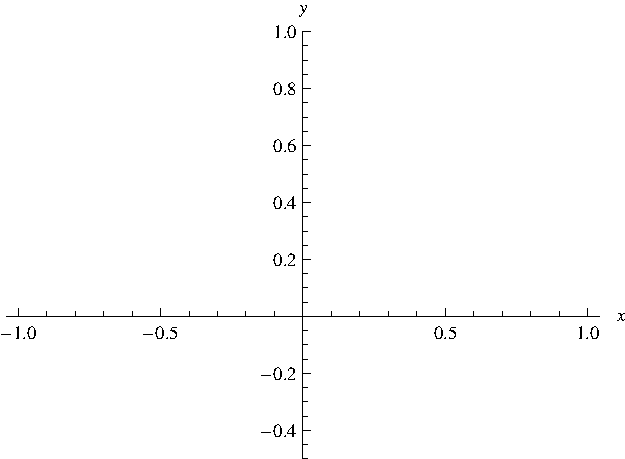
\includegraphics[height=4cm]{precalculus/pictures/01-01-ex-08a.pdf}%
%}%
%\only<handout:0| 2>{%
%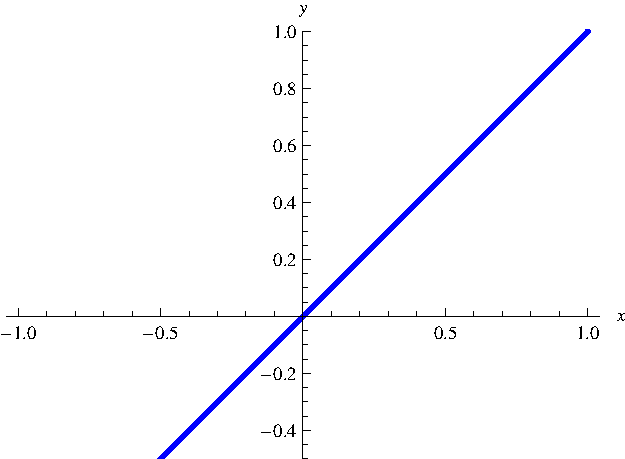
\includegraphics[height=4cm]{precalculus/pictures/01-01-ex-08b.pdf}%
%}%
%\only<handout:0| 3>{%
%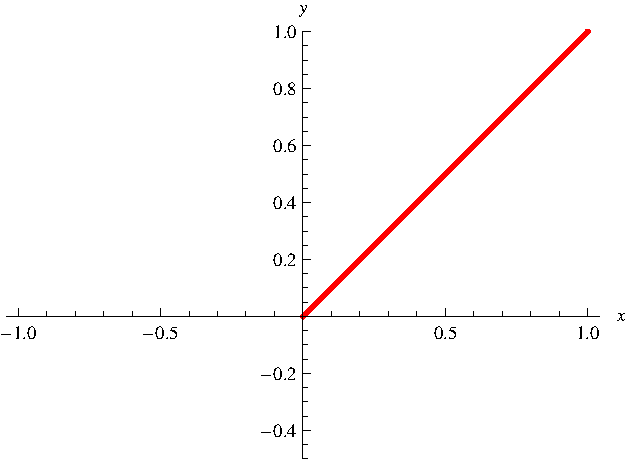
\includegraphics[height=4cm]{precalculus/pictures/01-01-ex-08c.pdf}%
%}%
%\only<handout:0| 4>{%
%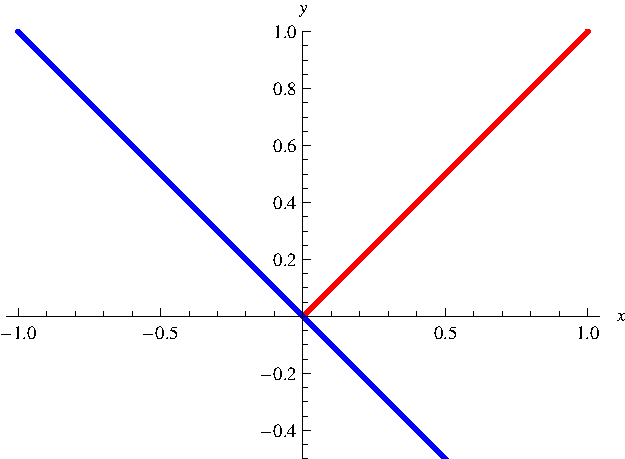
\includegraphics[height=4cm]{precalculus/pictures/01-01-ex-08d.pdf}%
%}%
%\only<handout:1-| 5>{%
%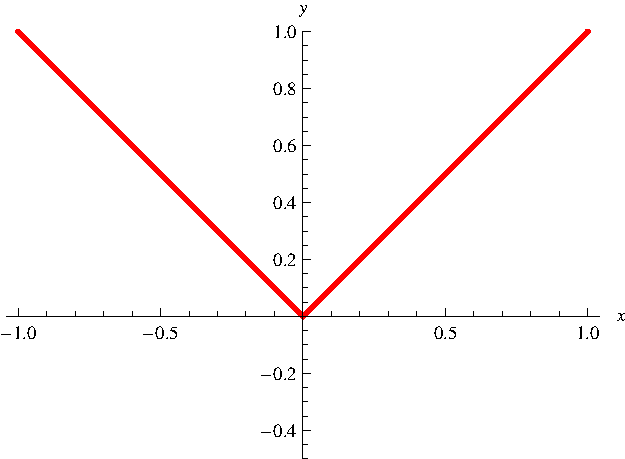
\includegraphics[height=4cm]{precalculus/pictures/01-01-ex-08e.pdf}%
%}%
\end{center}
\end{example}
\end{frame}
% end module absolute-value 
